
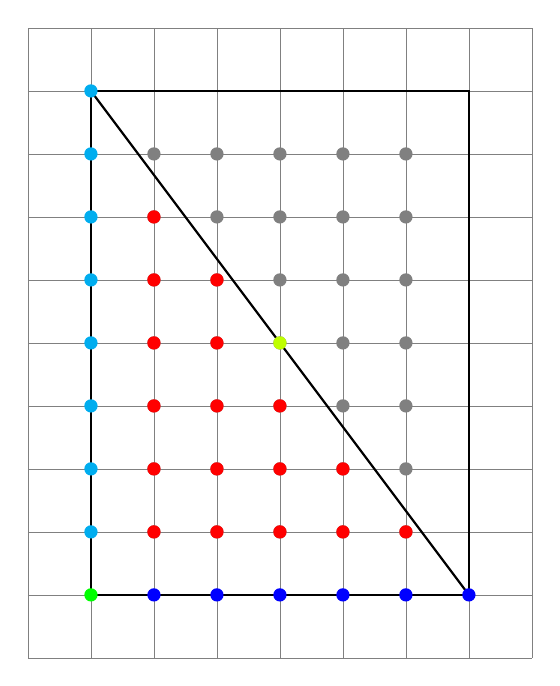
\begin{tikzpicture}[scale=.8]
  \draw[gray, very thin] (0,0) grid (8,10);
  \draw[thick] (1,1) rectangle (7,9);
  \draw[thick] (1,9) -- (7,1);
  \foreach \x in {2,3,4,5,6} {
    \foreach \y in {2,3,4,5,6,7,8} { \fill[gray] (\x,\y) circle (3pt); }
  }
  \foreach \x/\y in {
      2/2,2/3,2/4,2/5,2/6,2/7,3/2,3/3,3/4,3/5,3/6,4/2,4/3,4/4,5/2,5/3,6/2} {
    \fill[red] (\x,\y) circle (3pt); }
  \foreach \x in {2,...,7} { \fill[blue] (\x,1) circle (3pt); }
  \foreach \y in {2,...,9} { \fill[cyan] (1,\y) circle (3pt); }
  \fill[green] (1,1) circle (3pt);
  \fill[lime] (4,5) circle (3pt);
\end{tikzpicture}
